\chapter{Modell 1: YOLOX}\label{chap:yolox}
\section{Architektur}
\begin{figure}[h]
	\centering
	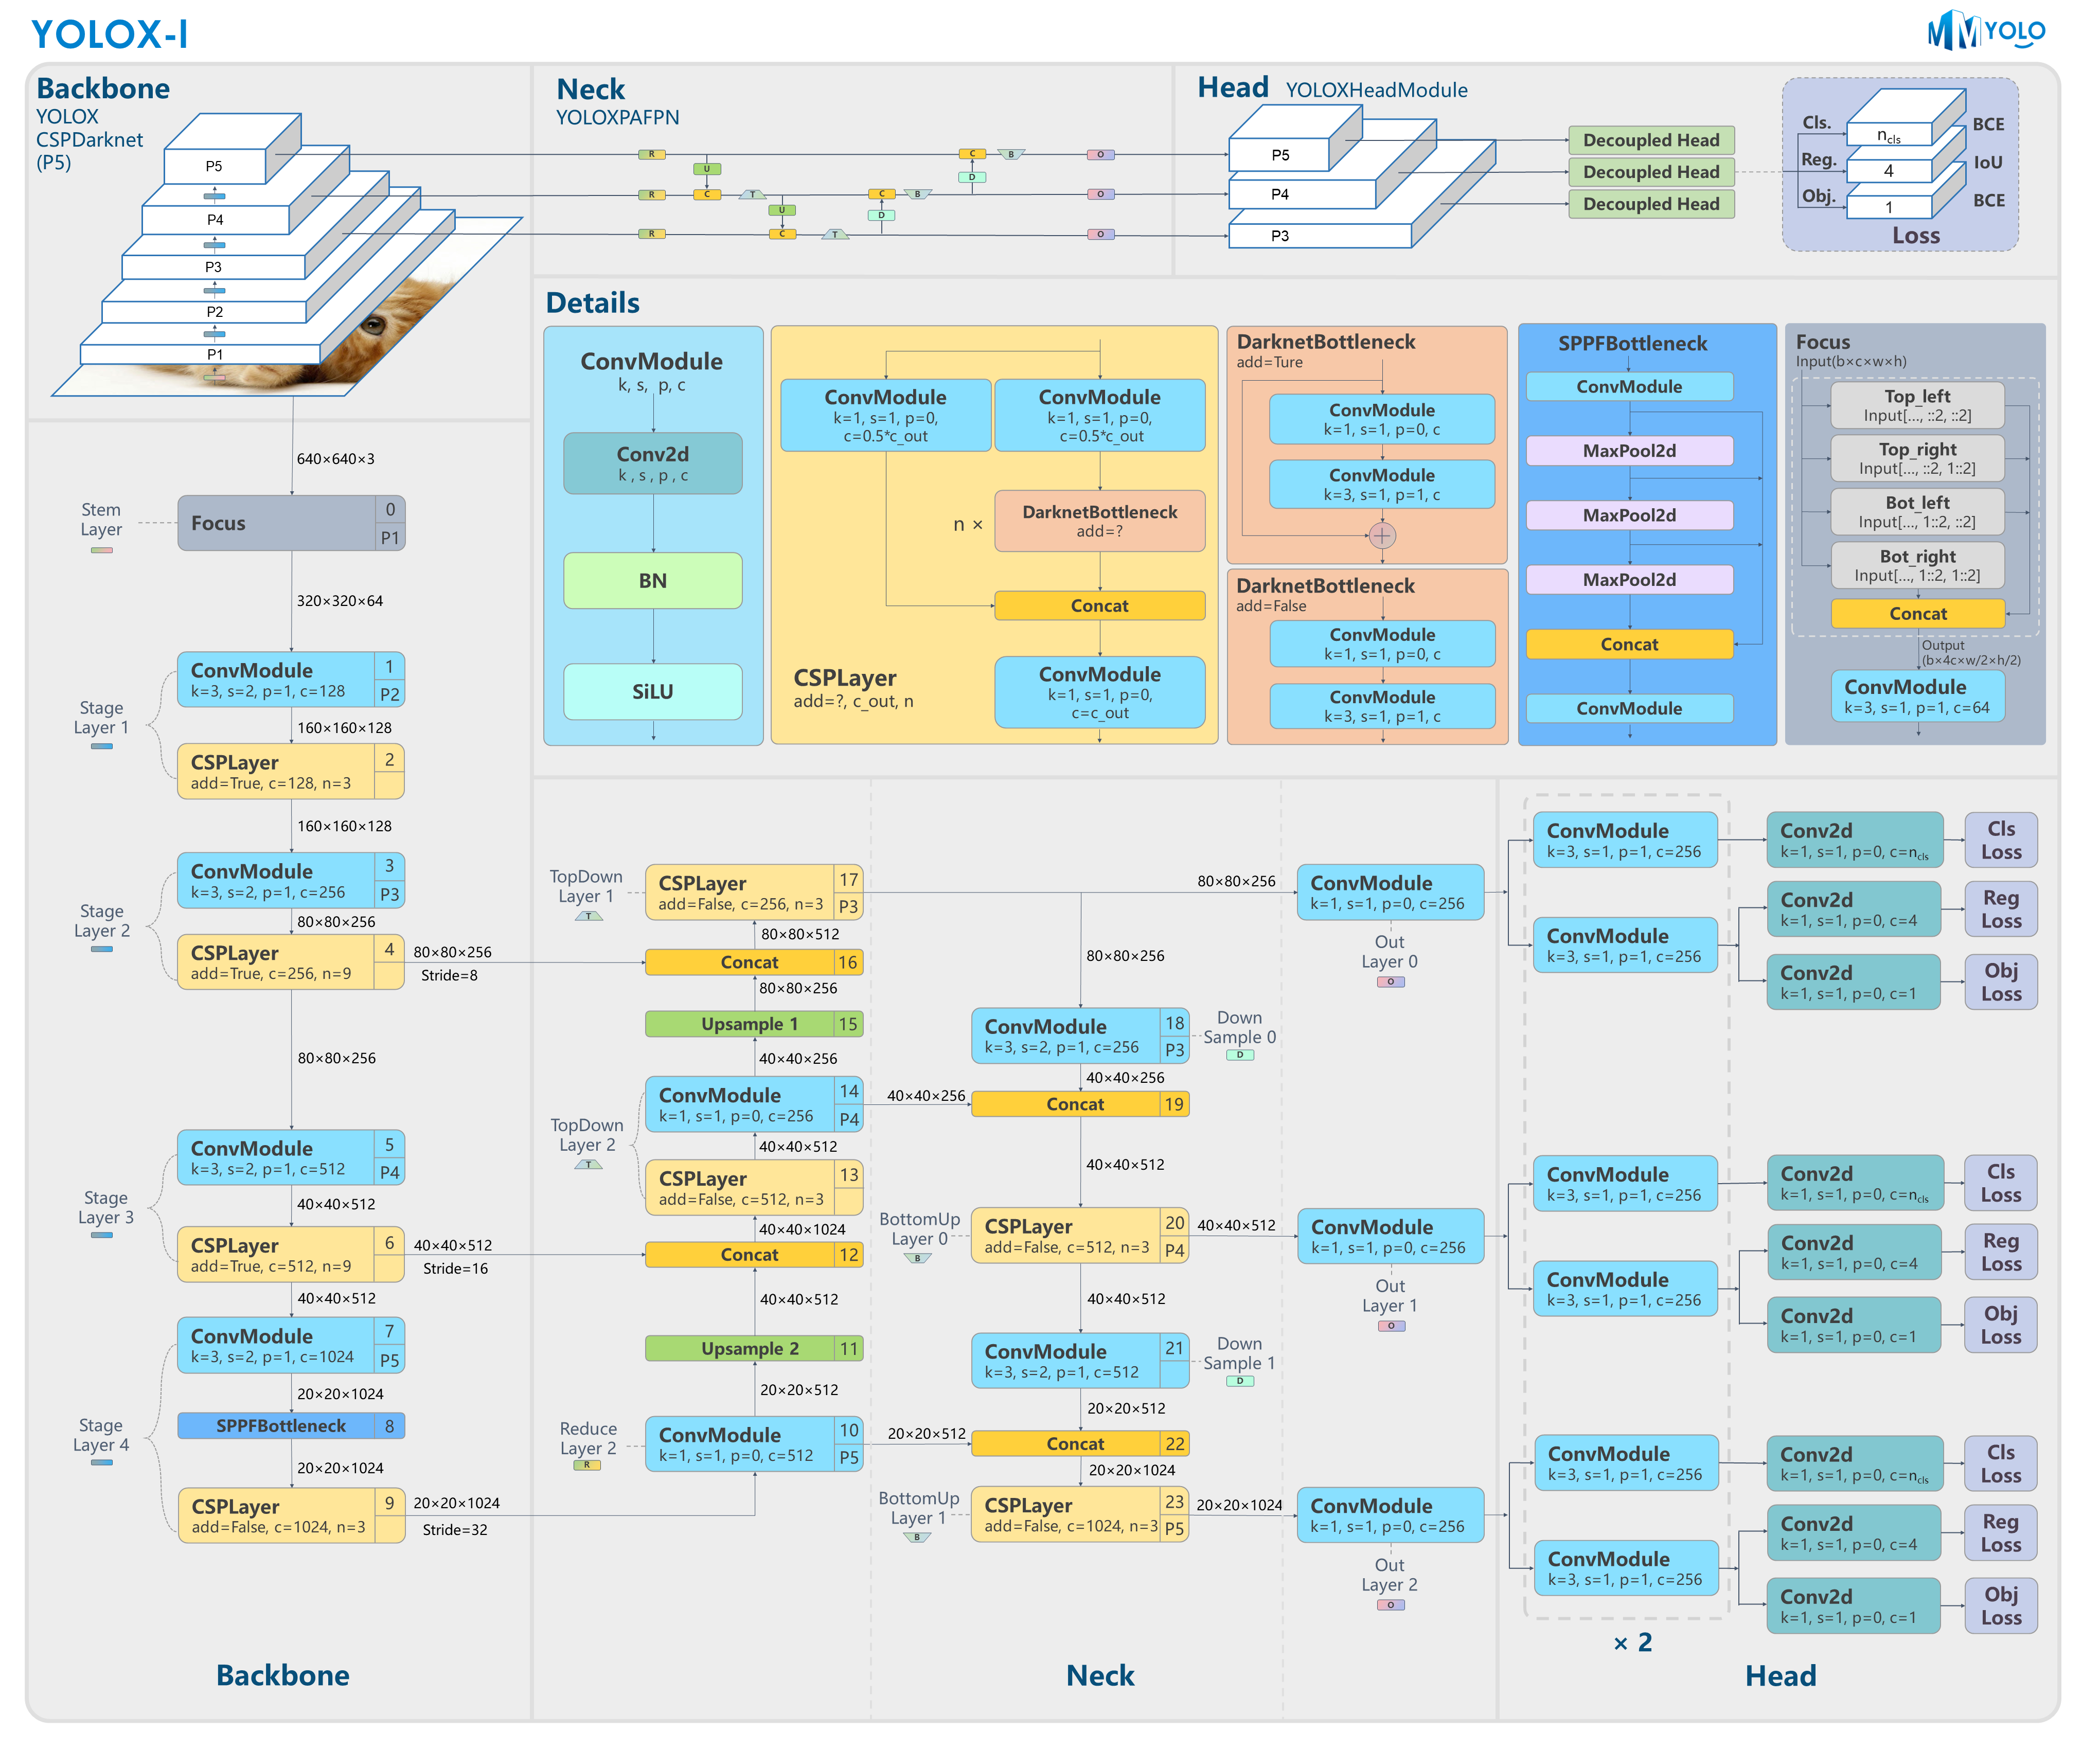
\includegraphics[width=0.8\linewidth]{yoloxArchitecture.png}
	\caption[Übersicht über die Architektur von YOLOX]{Übersicht über die Architektur von YOLOX. Quelle: \cite{yoloArchitecture, yoloxPaper, yoloxGitHubRepo}}
	\label{fig:yoloxArchitecture.png}
\end{figure}

Die YOLOX Architektur besteht aus einem Backbone-Netz, dem Neck und einem Head.

Das \textbf{Backbone}-Netzwerk ist für die Extraktion der Merkmale aus dem Bild verantwortlich. YOLOX verwendet das CSPDarknet als Backbone, um Merkmale auf 3 verschiedenen Maßstäben zu extrahieren. Die erste Ausgabe hat eine Dimension von ($H/8$x$W/8$x$256$), die Zweite eine Dimension von ($H/16$x$W/16$x$512$) und die Letzte eine Größe von ($H/32$x$W/32$x$1024$). Die beiden Parameter H und W sind die Höhe und Breite der Eingabe. Diese drei Ausgänge werden an das Neck weitergegeben. Durch die unterschiedlichen Skalierungen kann das Netz Merkmale für verschiedene Größen erzeugen. Der 256-Kanal-Ausgang extrahiert Merkmale mit einer kleineren Skalierung, während der 1024-Kanal-Ausgang Merkmale mit einer größeren Skalierung extrahiert. Mit zunehmender Tiefe des Netzes werden die Feature-Maps kleiner. Dadurch bleibt weniger Information von dem Originalbild erhalten. Die steigende Anzahl der Kanäle soll diesem Effekt entgegenwirken.

Die Ausgaben aus dem Backbone werden im CSP-Pyramid-\textbf{Neck} zu einer Merkmalspyramide verarbeitet, um Objekte unterschiedlicher Größen zu erkennen. Die drei verschiedenen Ausgaben werden wieder miteinander verrechnet (Faltung, Upsampling, Konkatenieren), um sie zu verbinden. Anschließend werden sie mit einem CSP-Layer auf drei unterschiedliche Dimensionen reduziert, um die Ergebnisse in den Head zu geben.

Der \textbf{Head} ist die Ausgabeschicht des Netzwerks und enthält die Detektionskomponente. YOLOX verwendet einen Decoupled Head, der aus zwei Teilen besteht. Dieser Mechanismus ist mit YOLOX neu eingeführt worden und wird in Kapitel \ref{decoupledHead} beschrieben.


\subsection{Decoupled Head}\label{decoupledHead}
Der Decoupled Head trennt die Vorhersage von Objekten und Bounding Boxes in zwei Zweige auf. Zusätzlich zum Pfad der Bounding-Box wird dort der Konfidenzwert vorhergesagt. Bei den herkömmlichen YOLO-Netzwerken wird die Vorhersage (Klasse, Bounding Box und Konfidenzwert) in einer einzigen Vorhersage gemacht. Dies kann zu Schwierigkeiten bei der Erkennung von Objekten unterschiedlicher Größe führen. 

Wie in der Abbildung \ref{fig:decoupledHead} (unten) zu sehen ist, wird im Decoupled Head die Dimension des Eingangs durch eine 1x1-Faltung reduziert und anschließend in zwei Pfade aufgeteilt. Das bedeutet, dass das Modell zuerst die Präsenz von Objekten vorhersagt und in einem parallelen Zweig die Bounding-Box-Koordinaten und den Objektscore für die erkannten Objekte berechnet. Dieser Head wird für jede drei FPN-Merkmale ausgeführt. \cite{yoloxExplanationHowWorks}

Die drei Tensorausgaben von YOLOX enthalten die gleichen Informationen wie die Ausgänge des großen Tensors von YOLOv3:
\begin{itemize}
\item Cls: Die Klasse jeder Bounding Box
\item Reg: Die 4 Teile der Bounding Box
\item Obj: Wie sicher ist das Netzwerk, dass innerhalb der Bounding Box ein beliebiges Objekt ist
\end{itemize}


\begin{figure}[h]
	\centering
	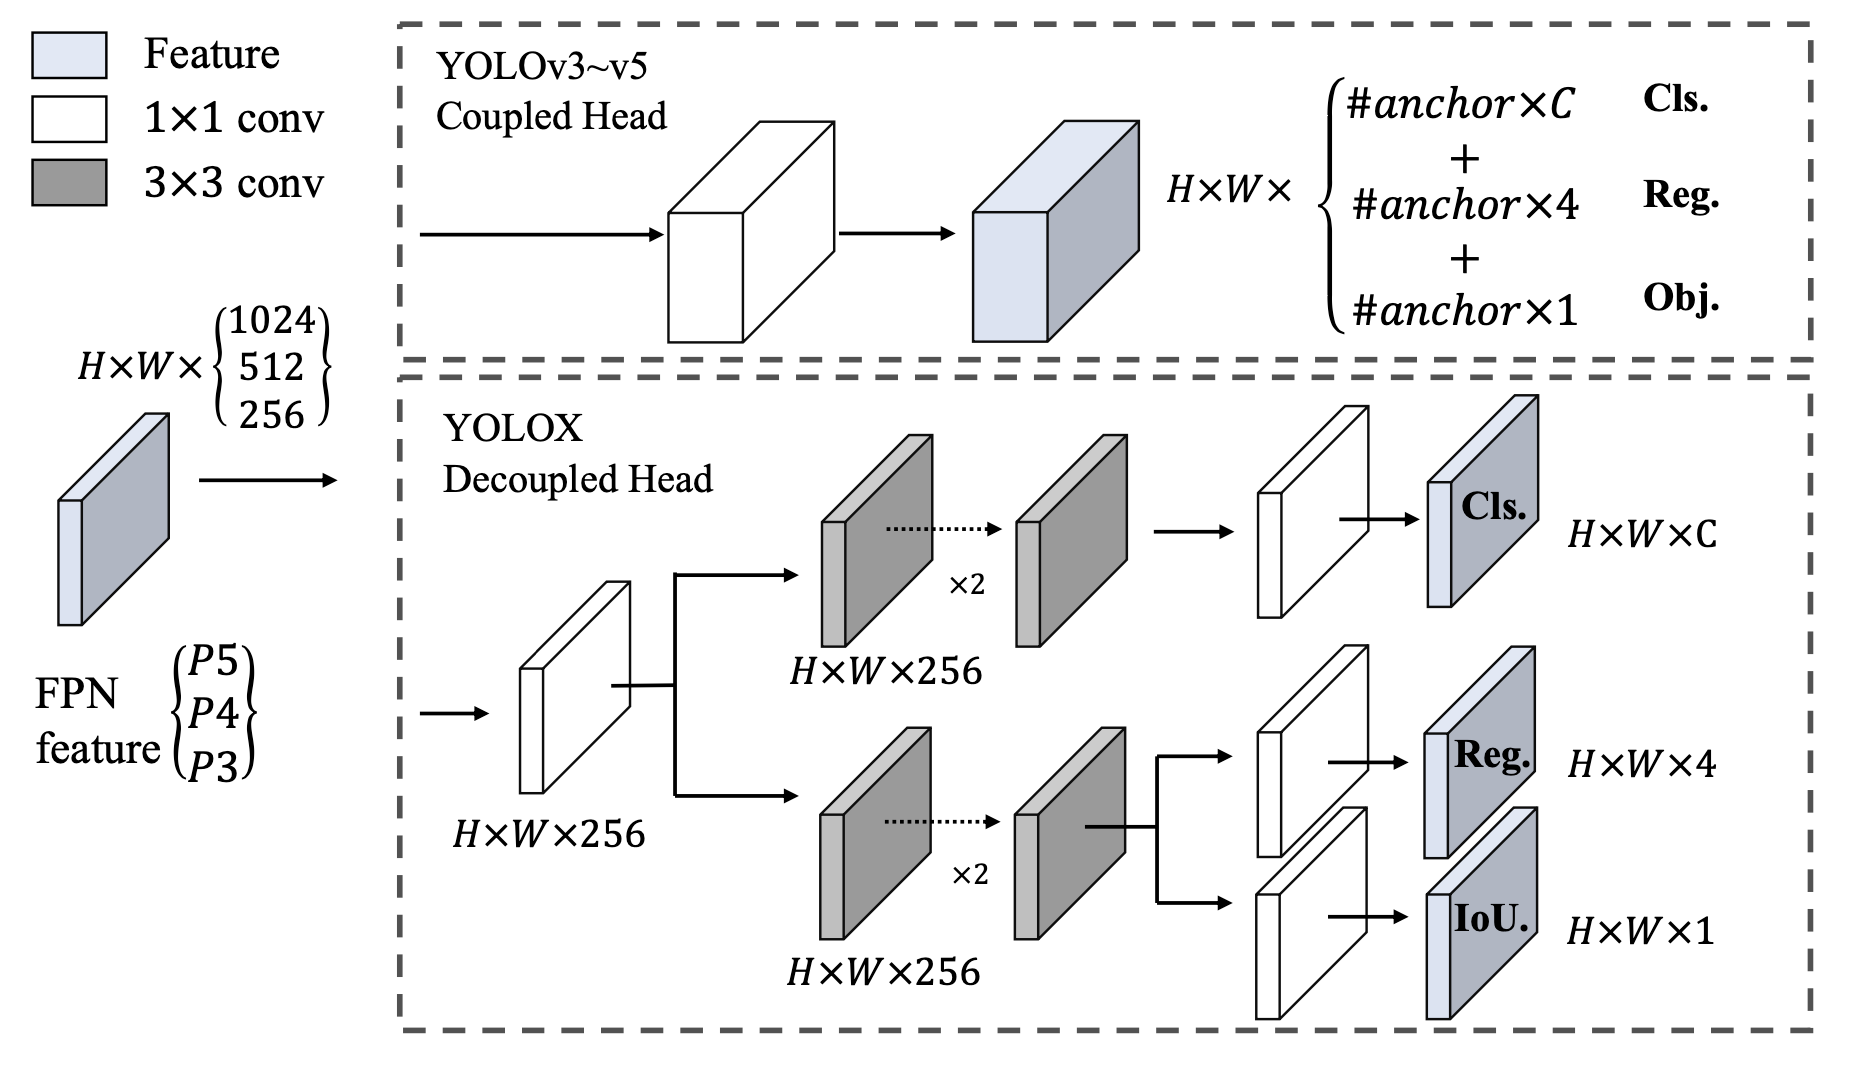
\includegraphics[width=0.55\linewidth]{decoupledHead.png}
	\caption[Illustration des Unterschieds zwischen dem Yolov3-Head und dem neuen Decoupled-Head ]{Illustration des Unterschieds zwischen dem YOLOv3-Head und dem neuen Decoupled-Head Quelle: \cite{yoloxPaper}}
	\label{fig:decoupledHead}
\end{figure}




\subsection{Anchor Free Prediction}



\subsection{SimOTA Label Assignment}


\subsection{Advanced Augmentation}


\section{Verlustfunktion}



\section{Modellauswertung}